\documentclass[a4paper,runningheads]{llncs}
\usepackage[T1]{fontenc}
\usepackage{booktabs}
\usepackage{graphicx}
\usepackage{microtype}
\usepackage{multirow}
\usepackage{url}
\usepackage{xcolor}
\usepackage{amsmath}
\usepackage{array}
\usepackage{placeins}
\usepackage[hidelinks]{hyperref}
\renewcommand\UrlFont{\color{blue}\rmfamily}
\urlstyle{rm}
\graphicspath{{figures/}}
\makeatletter\def\institutename{\par\begingroup\parskip=\z@\parindent=\z@\setcounter{@inst}{1}\def\and{\par\stepcounter{@inst}\noindent\textsuperscript{\the@inst}\enspace\ignorespaces}\setbox0=\vbox{\def\thanks##1{}\@institute}\ifnum\c@@inst=1\relax\gdef\fnnstart{0}\else\xdef\fnnstart{\c@@inst}\setcounter{@inst}{1}\noindent\textsuperscript{\the@inst}\enspace\fi\ignorespaces\@institute\par\endgroup}\makeatother
\renewcommand{\orcidID}[1]{\unskip\textsuperscript{[#1]}}
\newcommand{\repeatthanks}{\textsuperscript{$\star$}}
\newcommand{\tool}{\textsc{EvalGauge}}
\begin{document}

\title{EvalGauge: Auditing Typed Scoring Semantics in Scientific VQA Benchmarks}
\titlerunning{EvalGauge: Auditing Typed Scoring Semantics}
\author{Qing Mu\inst{1}\thanks{Equal contribution.}\orcidID{0009-0004-9571-2728} \and
Jiani Zheng\inst{2}\repeatthanks\orcidID{0009-0006-2835-5147}}
\authorrunning{Q. Mu and J. Zheng}
\tocauthor{Qing Mu and Jiani Zheng}
\institute{The Chinese University of Hong Kong, Shenzhen, Shenzhen, China\\
\email{qingmu@link.cuhk.edu.cn} \and
Tencent, Shenzhen, China\\
\email{ninajnzheng@tencent.com}}
\maketitle

\begin{abstract}
Automatic evaluation determines which model outputs count as correct in a multimedia benchmark. We show that scientific VQA scorers can change this definition through hidden choices about extraction, types, units, intervals, lists, and fallback rules. \tool{} compiles released annotations and scoring rules into typed contracts, then generates paired probes that preserve or violate the declared answer meaning. Across every public row of MeasureBench and ChartQAPro, it exposes order-dependent alternatives, type and dimension confusion, and invalid fallback credit. Reversing only the serialization of legal clock alternatives changes 168 decisions on 84 MeasureBench rows, while its official scorer accepts 2,612 contract-breaking probes. ChartQAPro assigns nonzero credit to 760 of 3,170 invalid probes. Rescoring all 4,884 MeasureBench-released predictions changes 35 labels on 33 rows. Within this changed-label set, two blinded reviewers show strong agreement ($\kappa=0.826$), and adjudicated judgments most often align with the source-declared Core policy (24/34 determinate cases).
\keywords{scientific multimedia evaluation \and visual question answering \and benchmark auditing \and answer contracts \and trustworthy multimedia evaluation}
\end{abstract}

\begin{figure}[!t]
  \centering
  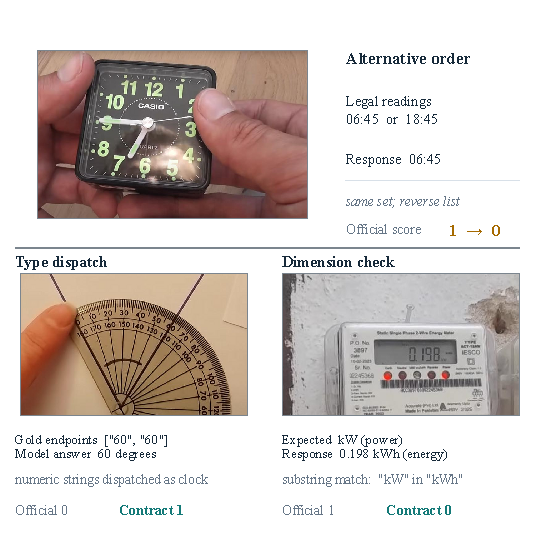
\includegraphics[width=\textwidth]{fig0_teaser.pdf}
  \caption{Three evaluator failures: order-sensitive legal alternatives, numeric/clock type dispatch, and energy--power substring confusion. Image crops are adapted from MeasureBench~\cite{lin2026measurebench} under CC BY-SA 4.0; cropping and annotations are ours, with source and license details in the artifact.}
  \label{fig:teaser}
\end{figure}

\section{Introduction}
Multimedia benchmarks increasingly ask models to read instruments, reason over charts, and return compact scientific or numerical answers. MeasureBench contains 2,442 visual-measurement questions~\cite{lin2026measurebench}; ChartQAPro contains 1,948 questions over 1,341 real-world charts~\cite{masry2025chartqapro}. Their answers appear short, but their evaluators must decide what constitutes the same value, list, label, unit, interval, or final response. A prediction such as ``100 mL'' denotes a value, a physical dimension, a unit, and membership in one or more accepted intervals. A clock answer such as ``01:00'' is structured but is not interchangeable with the number 60.

An evaluator that dispatches on endpoint type, matches units by substring, or pairs alternatives with \texttt{zip} can reject equivalent answers and accept scientifically invalid ones. It therefore changes the operational definition of correctness while the model output remains fixed. These decisions enter published VLM comparisons, category-level analyses, and the image--question pairs labeled as hard cases.

\tool{} turns each released answer specification into a typed scoring contract. From it, we generate equivalent answers that should retain credit and invalid answers that should not, then compare the released and reference scorers. This is an application of metamorphic testing~\cite{segura2016survey}, with relations derived from answer types and matching rules rather than generic input perturbations~\cite{ribeiro2020checklist}.

We ask three questions: \textbf{RQ1}, what executable assumptions define correctness in scientific VQA scorers? \textbf{RQ2}, which assumptions break answer equivalence or admit invalid credit? \textbf{RQ3}, how do these failures affect released model outputs?

Our contributions are:
\begin{itemize}
  \item evidence that scorer control flow changes scientific answer identity across two evaluator families, including order-dependent alternatives and credit for type- or dimension-invalid responses;
  \item \tool{}, which represents benchmark-specific extraction and matching rules as typed contracts and tests them with paired valid and invalid probes;
  \item full-row audits over 4,390 public examples, four-upstream parity, complete rescoring of 4,884 released predictions, and blinded dual review of every changed label.
\end{itemize}

\section{Background and Related Work}
\textbf{Scientific and chart VQA evaluation.} MeasureBench contains 1,272 real-world and 1,170 synthetic instrument-reading examples~\cite{lin2026measurebench}. Scientific VQA consistency has been tested under answer-choice permutation and question paraphrase~\cite{quan2025scientificvqa}; accuracy alone can miss unstable behavior. Scene-text, document, and expert VQA diversify answer forms~\cite{biten2019stvqa,mathew2021docvqa,yue2024mmmu}. ChartQA established visual and logical chart reasoning~\cite{masry2022chartqa}; ChartQAPro expands it to real-world questions and combines relative tolerance, ordered lists, exact types, and ANLS fallback~\cite{masry2025chartqapro}. These two released scorers give us complementary quantity and hybrid answer algebras.

\textbf{Robustness and evaluation in multimedia.} Recent MMM studies measure whether perturbations preserve model behavior: query edits expose brittle CLIP rankings~\cite{tran2026brittleness}, PRSM tests paraphrase stability~\cite{schlegel2026prsm}, and GaslightingBench-R tests resistance to adversarial negation~\cite{zhu2026gaslighting}. Image2Text2Image evaluates captions by reconstructing images and comparing visual features~\cite{huang2025image2text2image}. Facet-Probe audits model-level order sensitivity by reordering options, evidence chunks, document ranks, image sets, and mixed-modality evidence~\cite{paruchuri2026sameevidence}. Our alternative-order probe fixes the multimedia evidence and model response; only the scorer-side serialization of the same legal answer set changes.

\textbf{Learned and audited VQA scoring.} LAVE casts VQA evaluation as LLM-based answer rating and improves agreement with human judgments for open-ended candidate--reference pairs~\cite{manas2024lave}. Ye et al. audit six VLMs and six short-answer benchmarks with human-validated semantic judges; their deterministic bidirectional repair recovers evaluator-sensitive undercount~\cite{ye2026vqascore}. Scientific scalar answers additionally carry type, dimension, unit, interval, container, and legal-alternative semantics executed by released code. \tool{} audits this declared-answer layer, localizes faults from schema handling through aggregation, and tests invalid credit as well as valid-answer rejection. Each decision has a deterministic execution trace.

\begin{table}[t]
\centering
\caption{Technical scope of representative VQA validity methods.}
\label{tab:related-scope}
\footnotesize
\setlength{\tabcolsep}{2.0pt}
\renewcommand{\arraystretch}{1.08}
\begin{tabular}{@{}>{\raggedright\arraybackslash}p{0.16\textwidth}>{\raggedright\arraybackslash}p{0.17\textwidth}>{\raggedright\arraybackslash}p{0.20\textwidth}>{\raggedright\arraybackslash}p{0.18\textwidth}>{\raggedright\arraybackslash}p{0.21\textwidth}@{}}
\toprule
Work & Audited object & Structure & Oracle/control & Failure signal and locus\\
\midrule
LAVE~\cite{manas2024lave} & Learned answer rater & Free-form candidate/reference meaning & Human-rating agreement & Rating--human disagreement\\
Ye et al.~\cite{ye2026vqascore} & Natural response and context & Scalar, readout, identifier, multi-span & Human-validated semantic judge & False rejection; output/reference form\\
Facet-Probe~\cite{paruchuri2026sameevidence} & Model-input ordering & Options, chunks, documents, images & Cross-order flips; same-order control & Generation-order instability\\
\tool{} & Released scorer; fixed response & Type, unit, interval, list, alternatives & Source-compiled contract; blinded case review & Valid rejection and invalid credit; schema--aggregation\\
\bottomrule
\end{tabular}
\end{table}

\textbf{Metrics as structured semantics.} Structured-prediction metrics choose an output type and matching algebra~\cite{chen2023unified}, and undocumented preprocessing can materially change results~\cite{chen2022reproducibility}. \tool{} represents dimensions, unit conversions, intervals, and extraction rules explicitly and reports why each prediction is accepted or rejected.

\textbf{Metamorphic and property-based testing.} Metamorphic testing is useful when individual outputs lack a convenient oracle~\cite{segura2016survey,chen2011metamorphic}; property-based testing generates inputs from declared invariants~\cite{claessen2000quickcheck}. We combine both: dataset-derived contracts supply exact oracles, relations alter representation or meaning, and fixed-seed fuzzing exercises implementation invariants.

\section{Typed Scoring Contracts}
\subsection{Fault loci and contract types}
For an annotation row $r$ and model response $y$, a multimedia benchmark score can be written as
\begin{equation}
S(r,y)=G\!\left(M\!\left(N(E(y)),C(A(r))\right)\right),
\end{equation}
where $A$ interprets the annotation, $C$ compiles legal answers, $E$ extracts a final response, $N$ normalizes it, $M$ compares it with the compiled rule, and $G$ aggregates the result. This factorization separates failures in schema handling, extraction, type routing, comparison, and aggregation. Benchmark-specific adapters expose these choices to a shared generator of valid and invalid probes.

The shared interface admits four contract forms:
\begin{equation}
\mathcal{C} ::= Q(\tau,d,U,I)\mid X(t,V)\mid L(\mathcal{C}_{1:m},\pi)\mid T(\phi),
\end{equation}
where $Q$ is a numeric or clock quantity with type $\tau$, dimension $d$, allowed units $U$, and closed intervals $I$; $X$ is an exact typed value; $L$ is a list with order policy $\pi$; and $T$ retains a benchmark's text-similarity rule $\phi$. A response is valid when its parsed content satisfies a legal branch under the selected scoring policy.

\begin{figure}[t]
  \centering
  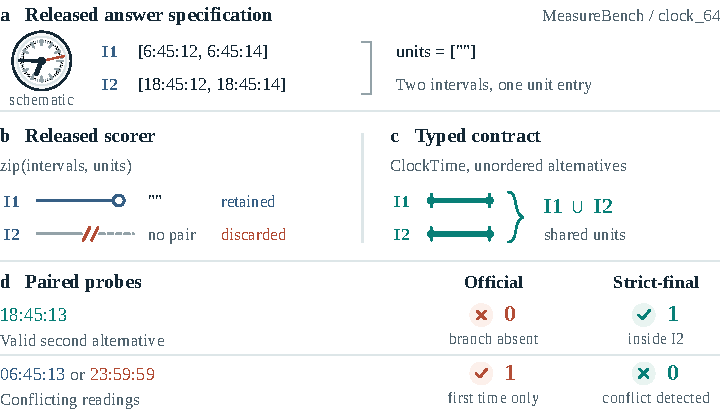
\includegraphics[width=\textwidth]{fig1_pipeline.pdf}
  \caption{Overview of \tool{}. Benchmark-specific scoring rules are compiled once and reused for paired probes and natural-output rescoring.}
  \label{fig:pipeline}
\end{figure}

\subsection{Compiling benchmark semantics}
The MeasureBench adapter maps numeric and clock annotations to $Q$ contracts. Numeric endpoints use decimal arithmetic; clocks require an explicit colon grammar; and multiple intervals form a disjunction. A flat unit list attached to several intervals is interpreted as a shared alias set, while the order-dependence test executes the released schema before this repair. The unit registry stores aliases, dimensions, scales, and offsets. It permits multiplicative conversion $x_b=ax$ and affine temperature conversion $x_b=ax+b$ only between registered units of the same dimension.

The ChartQAPro adapter maps year, multiple-choice, and fact answers to $X$; scalar answers to numeric $Q$ contracts with relative tolerance; list answers to $L$; and remaining text answers to $T$. Each adapter therefore retains its native comparison and aggregation rules rather than imposing one universal metric.

All reported profiles preserve the released final-answer extraction:
\begin{center}
\small raw response $\rightarrow$ released final segment $\rightarrow$ typed parse $\rightarrow$ contract match.
\end{center}
The extractor prioritizes \texttt{Answer:}/localized markers and then \verb|\boxed{}|; if neither exists, it returns the response. A broader final-marker extractor and whole-response matching are used only to measure extraction sensitivity.

The parser covers common numeric, clock, unit, and structured-answer forms, including fractions, scientific notation, and LaTeX units. Unit aliases use token boundaries; non-finite values are rejected. Each decision records the extracted segment, parsed quantities, matched branch, normalized value and unit, and rejection reason.

\subsection{Scoring policies and traces}
All profiles use typed endpoints, unordered alternatives, closed intervals, and the released final-answer extractor. \textbf{Core-final} restricts matches to source-declared units. \textbf{Physics-final} adds same-dimension conversions, while \textbf{Strict-final} also rejects conflicting expected-type quantities. We run each profile independently and retain its decision trace.

\section{Experimental Setup}
\subsection{Benchmarks and scorers}
MeasureBench has 2,442 rows and 2,887 numeric or clock branches~\cite{lin2026measurebench}. We reproduce its released FlagEvalMM scorer and current standalone implementation~\cite{measurebenchrepo2026}. Both agree with our reproduction on 88,189 executions over witnesses, probes, and model responses. The \emph{Numeric-string patch} changes only colon-free numeric-string endpoints to floats.

ChartQAPro contributes 1,948 rows with a different scoring algebra~\cite{masry2025chartqapro}. Its adapter covers 522 exact-type, 657 scalar-numeric, 19 ordered-list, and 750 text-similarity answers. Both the repository scorer and recommended VLMEvalKit implementation~\cite{duan2024vlmevalkit} agree with our reproduction on all 18,186 executions.

\subsection{Generated probes and metrics}
For MeasureBench, 44,566 contract-valid probes cover equivalent numeric notation, wrappers, unit aliases and conversions, schema variants, interval boundaries, and number--clock separation. Another 37,212 probes violate a boundary, unit, dimension, type, or response-consistency rule. Candidates that accidentally satisfy a different legal branch are discarded. ChartQAPro adds 9,093 cases over source answers, formatting, numeric tolerance, list structure, malformed numerics, and non-finite values.

\paragraph{Companion artifact.}
The complete relation registry, case-level decisions, review records,
and reproduction scripts are available in the companion
repository.\footnote{\url{https://github.com/mqingcs/EvalGauge}}

We track acceptance of source and canonical witnesses (SWAR and CCA), invariance under valid reformulations (MIR), and errors on valid and invalid probes (suite-FRR and suite-FAR). Case-, row-, and relation-level aggregates are reported in the artifact; main-paper rates are full-population case counts.

\subsection{Natural outputs and manual case audit}
We reproduce all 4,884 GPT-5 and Gemini-2.5-Pro predictions released with MeasureBench and additionally score 637 provenance-linked outputs from three contemporary VLMs. All reported policies operate after the released final-answer extractor.

Every Official--Strict label change undergoes two independent human reviews. Each reviewer sees only the image, question, raw released annotation, benchmark instruction, and model response, and assigns \emph{accept}, \emph{reject}, or \emph{ambiguous}. Compiled contracts, Official and Strict scores, fault attributions, and the other verdict are hidden. A finalized dual-scale rule requires every claimed final reading to satisfy its paired source interval. Before the second review began, Reviewer A re-judged seven affected cases under the finalized rule without access to Reviewer B's verdicts; provisional and finalized-SOP labels are both retained. A third reviewer independently adjudicated the three remaining disagreements from the same blinded materials. We report finalized-SOP agreement, Cohen's $\kappa$, disagreement types, and adjudicated profile alignment.

\section{Results}
\subsection{Cross-benchmark scorer semantics}
Table~\ref{tab:xbench} shows that the same contract interface supports interval- and unit-based measurement as well as a hybrid chart-QA scorer. Across both benchmarks, all 4,390 public rows compile into 90,871 cases; the reference implementations pass the complete declared suite, and combined upstream parity covers 106,375 executions without a mismatch.

\begin{table}[t]
\centering
\caption{Cross-benchmark execution. MeasureBench reports binary acceptance; ChartQAPro's official metric is soft, so invalid leakage denotes nonzero score.}
\label{tab:xbench}
\setlength{\tabcolsep}{3.2pt}
\begin{tabular}{lrrrr}
\toprule
Evaluator family & Rows & Cases & \shortstack{Source-witness\\full credit} & Invalid leakage\\
\midrule
MeasureBench & 2,442 & 81,778 & 96.12\% & 2,612/37,212\\
ChartQAPro & 1,948 & 9,093 & 99.38\% & 760/3,170\\
\midrule
Total & 4,390 & 90,871 & -- & --\\
\bottomrule
\end{tabular}
\end{table}

ChartQAPro rejects full credit for 12 direct source witnesses: one non-finite string token and 11 bracketed source lists with unquoted elements. On the negative side, 760 of 3,170 contract-breaking probes receive nonzero official credit (23.97\%). Two mechanisms dominate. First, both upstream implementations compute an exact-match switch for Fact Checking and Multi Choice but do not forward it to the scorer; ANLS therefore gives partial credit to 292 of 522 extra-token probes over exact-type rows. Second, a failed numeric parse falls through to text similarity, crediting 452 of 657 malformed numeric suffixes. The official aggregate averages these soft scores, so the leakage directly enters reported accuracy. This independent evaluator family reproduces the same higher-level failure pattern as MeasureBench: answer type and fallback control flow are benchmark semantics.

\subsection{Valid-answer instability and invalid credit}
\paragraph{Full contract audit.}
Table~\ref{tab:main} shows a wide gap between annotation-local success and scorer invariance. The official scorer accepts 96.12\% of source-format witnesses but only 84.66\% of canonical witnesses. It rejects 25.65\% of source- or representation-preserving probes and 28.20\% of physical-equivalence extensions; the pooled 26.03\% is reported only as an all-probe aggregate. It also credits 7.02\% of contract-breaking probes. The narrow patch fixes all 14 numeric-string source witnesses and raises valid-reformulation invariance by 4.47 points, yet leaves invalid credit unchanged. Row- and relation-level aggregates are reported in the artifact.

\begin{table}[t]
\centering
\caption{MeasureBench generated-probe audit. Top: scorer-level rates (\%). Bottom: official rejection by positive claim scope; physical conversions are semantic extensions.}
\label{tab:main}
\setlength{\tabcolsep}{4.2pt}
\begin{tabular}{lrrrrr}
\toprule
Scorer & SWAR & CCA & MIR & FRR & FAR\\
\midrule
Official & 96.12 & 84.66 & 85.48 & 26.03 & 7.02\\
Numeric patch & 96.61 & 85.14 & 89.94 & 21.20 & 7.02\\
\bottomrule
\end{tabular}

\vspace{4pt}
\footnotesize
\begin{tabular}{lrrr}
\toprule
Positive claim scope & Valid probes & Rejected & Rate (\%)\\
\midrule
Source-/representation-preserving & 37,911 & 9,725 & 25.65\\
Physical-equivalence extension & 6,655 & 1,877 & 28.20\\
\bottomrule
\end{tabular}
\end{table}

The 112 branch-level source-witness failures reveal four concrete implementation classes. Fourteen are numeric strings routed to the clock parser; 86 are clock branches affected by flat-unit alternative truncation (including three with signed clock components); three have reversed bounds; and nine pressure answers contain exponent digits such as \texttt{kgf/cm\textasciicircum2}, which the number extractor mistakes for the final predicted value. The narrow repair removes only the first class, leaving 98 failures.

\paragraph{Representation and order.}
Common equivalents also fail: only 0.60\% of scientific-notation variants are accepted, while schema-equivalent containers trigger 1,534 official exceptions. Conversion cases are reported as semantic-coverage extensions rather than implementation defects; relation-level results are in the artifact.

Alternative permutation exposes a separate schema interaction. Of 141 flat-unit clock rows, 84 have mismatched interval and unit cardinalities, so released \texttt{zip} execution discards 86 declared alternatives. Reversing only interval serialization produces 168 binary-score flips across those 84 rows while candidate answers and legal interval sets remain unchanged. The flip occurs in the released schema itself, regardless of how shared units are repaired; treating alternatives as an unordered disjunction removes the dependence.

\paragraph{Invalid-answer credit.}
Among 37,212 contract-breaking probes, the official scorer credits 2,612 (7.02\%). Substring matching credits 1,898 extended-unit responses because a short alias can occur inside a longer invalid token. Selecting the first clock or last number credits another 452 contradictory multi-value responses. The numeric-string patch leaves these invalid credits unchanged.

\begin{table}[t]
\centering
\caption{Distinct scoring algebras expose recurring fault loci. Counts are generated probes unless labeled as source witnesses or score flips; response handling covers extraction and aggregation.}
\label{tab:fault-matrix}
\footnotesize
\setlength{\tabcolsep}{3.2pt}
\begin{tabular}{>{\raggedright\arraybackslash}p{0.16\textwidth}>{\raggedright\arraybackslash}p{0.36\textwidth}>{\raggedright\arraybackslash}p{0.36\textwidth}}
\toprule
Fault locus & MeasureBench & ChartQAPro\\
\midrule
Schema & 168 score flips under alternative reordering & 11 source lists lose full credit\\
Type routing & 14 numeric strings treated as clocks & 292/522 exact-answer suffixes gain ANLS credit\\
Comparison & 1,898 extended unit tokens accepted & 452/657 malformed numerics fall back to ANLS\\
Response handling & 452 contradictory multi-value answers accepted & Soft-element mean propagates fallback credit\\
\bottomrule
\end{tabular}
\end{table}

\subsection{Consequences for released predictions}
MeasureBench releases complete GPT-5 and Gemini-2.5-Pro predictions for both benchmark splits. We rescore all 4,884 answers and exactly reproduce the published rounded accuracies. Strict-final changes 35 labels on 33 unique rows: 28 official rejections become accepts, while seven official accepts are removed. Six of the 28 recoveries are already fixed by the numeric-string patch; 22 require broader quantity semantics. The published model order remains unchanged.

The policy ladder locates these changes: Core alters 68 labels, Physics recovers 53, and Strict removes 12. After Reviewer A re-judged the seven cases affected by the finalized dual-scale SOP, the reviewers agree on 32/35 model-answer cases (91.43\%; three-label Cohen's $\kappa=0.826$). All three residual disagreements carry a source-issue flag: one concerns image readability and two concern paired-scale interval consistency. The third reviewer adjudicated these cases, yielding 20 accepts, 14 rejects, and one image-ambiguous case.

Within this selected transition set, Core-final has the highest human alignment at 24/34 determinate cases (70.6\%), compared with 21 for the numeric patch, 19 for Strict, 17 for Physics, and 15 for Official. The pattern is clearer when cases are grouped by claim scope: adjudicated judgments support Core in 14/19 source-declared cases and Strict in 3/4 response-safety cases, but Physics in only 2/10 conversion-extension cases. This supports reporting registered conversions as semantic coverage rather than universal bug fixes. Both reviewers also independently flag two dual-scale source annotations as internally inconsistent.

\begin{table}[t]
\centering
\caption{Representative transitions from the blinded dual review. Each row received matching independent verdicts; source issues were flagged separately.}
\label{tab:natural-cases}
\footnotesize
\setlength{\tabcolsep}{2.7pt}
\begin{tabular}{>{\raggedright\arraybackslash}p{0.17\textwidth}>{\raggedright\arraybackslash}p{0.22\textwidth}c>{\raggedright\arraybackslash}p{0.37\textwidth}}
\toprule
Case & Released response & \shortstack{Official\\$\to$Strict} & Human review\\
\midrule
Protractor 3 & 60$^{\circ}$ & $0\to1$ & Unanimous accept: a numeric-string endpoint was routed as a clock\\
Pressure gauge 35 & 144 psi (or 10.4 bar) & $1\to0$ & Unanimous reject: the paired final readings conflict\\
Thermometer 13 & 24$^{\circ}$C (76$^{\circ}$F) & $0\to1$ & Unanimous accept: the $^{\circ}$C reading is supported; both reviewers flag the paired $^{\circ}$F source interval\\
\bottomrule
\end{tabular}
\end{table}

\begin{figure}[t]
  \centering
  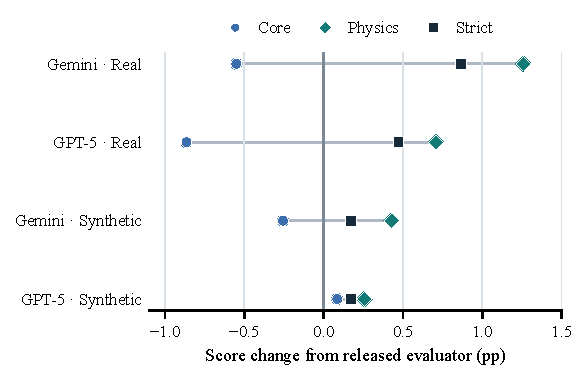
\includegraphics[width=0.82\textwidth]{fig6_public_rescoring.pdf}
  \caption{Score change from the released scorer. Core isolates representation and schema rules; Physics adds quantity conversion; Strict adds response consistency.}
  \label{fig:public}
\end{figure}

\FloatBarrier
\paragraph{Contemporary transfer.}
Across 637 contemporary outputs from Doubao Seed 2.1 Turbo, Gemini 3.6 Flash, and Qwen3-VL-8B, Strict-final differs from Official on nine events. The artifact reports the per-model breakdown.

A whole-response sensitivity check changes 486 Gemini decisions and reverses the aggregate order; all primary comparisons retain the released final-answer extractor~\cite{molfese2025right}.

\section{Discussion}
Across both benchmarks, the central failure is not a single parser bug. Scorer control flow determines which answer type is expected and which fallback can award credit. MeasureBench exposes this through alternative pairing and unit matching; ChartQAPro exposes it through exact-type and numeric fallbacks. These mechanisms change the operational definition of correctness while the image, question, and model response remain fixed.

The consequences appear at both item and aggregate levels. Among 34 determinate adjudicated cases, Core-final matches 24. Both reviewers independently identify two paired-scale source issues. The published model order is unchanged, showing that aggregate stability does not certify item validity or annotation consistency.

\tool{} targets closed-form answer layers whose types and comparison rules can be stated explicitly; subjective generation may still require human or learned evaluation. Because probe construction is annotation-driven, scorer revisions can be checked without rerunning the evaluated VLMs: maintainers execute source witnesses, equivalent reformulations, and invalid responses, then inspect only changed traces. For responsible multimedia AI, benchmark releases should specify the annotation schema, extraction policy, type router, comparator, and aggregation rule together and include these tests with the scorer.

\section{Conclusion}
\tool{} shows that answer scoring is a substantive part of scientific multimedia evaluation. Across MeasureBench and ChartQAPro, seemingly minor choices in representation, units, alternatives, and fallback behavior change which responses receive credit. Making these rules explicit yields reproducible scorer tests and more reliable, transparent model comparisons.

\begin{credits}
\subsubsection{\discintname}
The authors have no competing interests to declare that are relevant to the content of this article.
\end{credits}

\newpage
\bibliographystyle{splncs04}
\bibliography{references}
\end{document}
